\begin{summary}
    Ce premier chapitre sera l'occasion d'introduire le projet tel qu'il a été initié et de 
    détailler les outils et les méthodes envisagées pour son développement.
  \end{summary}

\section{Descriptif de la problématique}


Le pavage du plan avec des rectangle est un problème classique et déjà largement documenté,
mais je souhaite l'aborder par un aspect très concret : étant donné un nombre de tatamis, quelles sont les
configurations possibles.\\
\begin{center}
    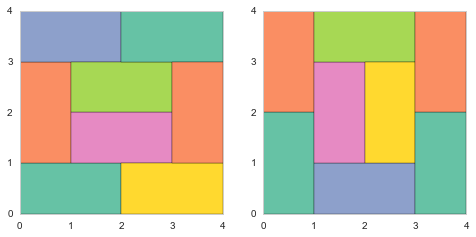
\includegraphics[width = 0.5\linewidth]{./images/pavage-par-tatamis.png}
\end{center}
C'est un problème que rencontre notamment toute personne qui se retrouve à devoir installer un dojo.
Il existe une contrainte de base qui est que 4 tatamis ne rejoignent jamais en un même coin. Mais ont peut
en ajouter d'autres : possibilité de demi-tatamis (carré), répartition des couleurs, répartition de l'usure...

\section{Ébauche de cahier des charges}

Utilisateur final : gestionnaire de dojo\\

L'interface utilisateur devra comprendre un menu de paramétrage basique : nombre de tatamis,
contraintes géométriques, contraintes d'aspect général; ainsi qu'un affichage des dispositions envisageables.\\

L'utilisateur devra pouvoir saisir :

\begin{itemize}
    \item le nombre et le type (entier/demis) de tatamis à disposition
    \item leurs dimensions
    \item leurs couleurs
    \item éventuellement leur état (on dispose de préférence les plus usés en périphérie)
    \item les dimensions du dojo
\end{itemize}

L'affichage proposera différentes disposition selon les contraintes imposées.

\section{Membres du projet}
